\section{ Result }
This chapter first goes through the results from the mobile application discovery survey. After that, the results from the usability tests are presented and lastly the decision-model that has been designed and implemented is shown. 

\subsection{Mobile application discovery survey}

A total of 94 people, 28 iPhone users and 66 Android users, participated in the internet survey. The age of the participants ranged from 20 to 73 years, with the median of the participants' age being 27 years. The average age was 32.7 years.  
In both cases of device used, only one person answered that they use internet searches to download applications. How Android users found information about applications can be seen in figure \ref{fig:android-info}. The same data for the iPhone users can be seen in figure \ref{fig:iphone-info}.

\begin{figure}[ht]
    \centering 
    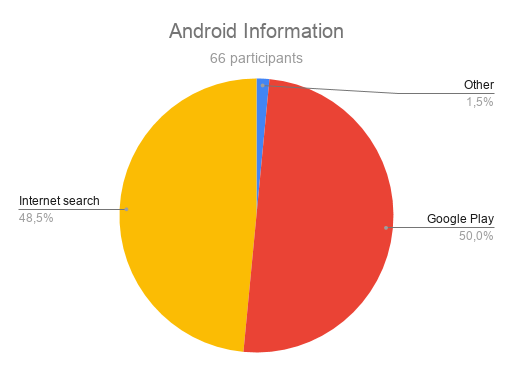
\includegraphics[width=0.9\textwidth]{img/Android_Information.png}
    \hfill
    \caption{\label{fig:android-info}{Android users' answers to "You just heard about a new smartphone application (app). Where do you turn when you want to find information about the app?".}}
\end{figure}

\begin{figure}[ht]
    \centering 
    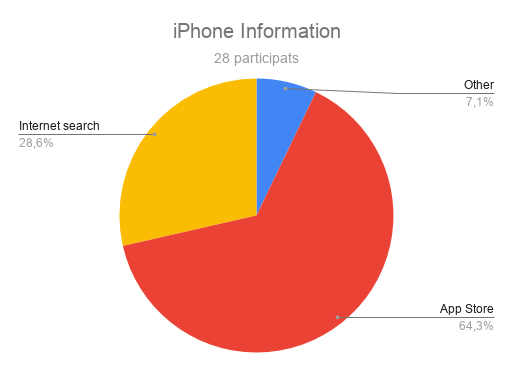
\includegraphics[width=0.9\textwidth]{img/iPhone_Information.png}
    \hfill
    \caption{\label{fig:iphone-info}{iPhone users' answers to "You just heard about a new smartphone application (app). Where do you turn when you want to find information about the app?".}}
\end{figure}

 The users on average answered that they spent more time on applications than browsing the web, but no statistical conclusion could be drawn from the questions on web browsing vs. application usage or security, as can be seen in appendix \ref{appendix:b}.
 
\subsection{Usability test}
The findings from the usability tests regarding user experienced is analyzed through the UEQ, SUS and the qualitative data gathered from the tests. There were a total of 18 tests, 5 iPhone users and 13 Android users.

\subsubsection{UEQ}

Two of the five categories of the UEQ got statistically significant results on a confidence level of 95\%: Attractiveness and Efficiency. Dependability and Stimulation had statistically significant results on a confidence level of 85\%. Due to this low value, in the first calculation, only the categories of Attractiveness and Efficiency were chosen to form the basis for the criteria UX in the model.

Perspicuity had no significant difference on any reasonable confidence level.

To quantify the results from the UEQ, the score for PWA was divided by the score for Native in the different categories. This provided a relative ratio between PWA and Native which was used to set the score for the criteria. The relative ratio score for the categories Attractiveness and Efficiency can be seen in table \ref{tab:relative-ratio1} The average for the two statistically significant categories was 0.62.

\begin{table}[ht]
    \centering
    \begin{tabular}{ |c|c| } 
        \hline
        \rowcolor{light-gray}
          & Relative Ratio Score \\
        \hline
        Attractiveness & 0.68 \\
        \hline
        Efficiency & 0.56 \\
        \hline
        Total Average: & 0.62 \\
        \hline
    \end{tabular}
    \caption{Relative ratio score from the 95\% statistically significant UEQ results}
    \label{tab:relative-ratio1}
\end{table}

The overall result from the UEQ, with the categories of low statistical significance included, can be seen in table \ref{tab:relative-ratio-all}. The total average was 0.77. The whole result without the relative ratio score can be found as a graph in figure \ref{fig:ueq-result}.

\begin{table}[ht]
    \centering
    \begin{tabular}{ |c|c| } 
        \hline
        \rowcolor{light-gray}
          & Relative Ratio Score \\
        \hline
        Attractiveness & 0.68 \\
        \hline
        Perspicuity & 1.14 \\
        \hline
        Efficiency & 0.56 \\
        \hline
        Dependability &  0.76 \\
        \hline
        Stimulation & 0.73 \\
        \hline
        Total Average: & 0.77 \\
        \hline
    \end{tabular}
    \caption{Relative ratio score from all UEQ results}
    \label{tab:relative-ratio-all}
\end{table}

\begin{figure}[ht]
    \centering 
    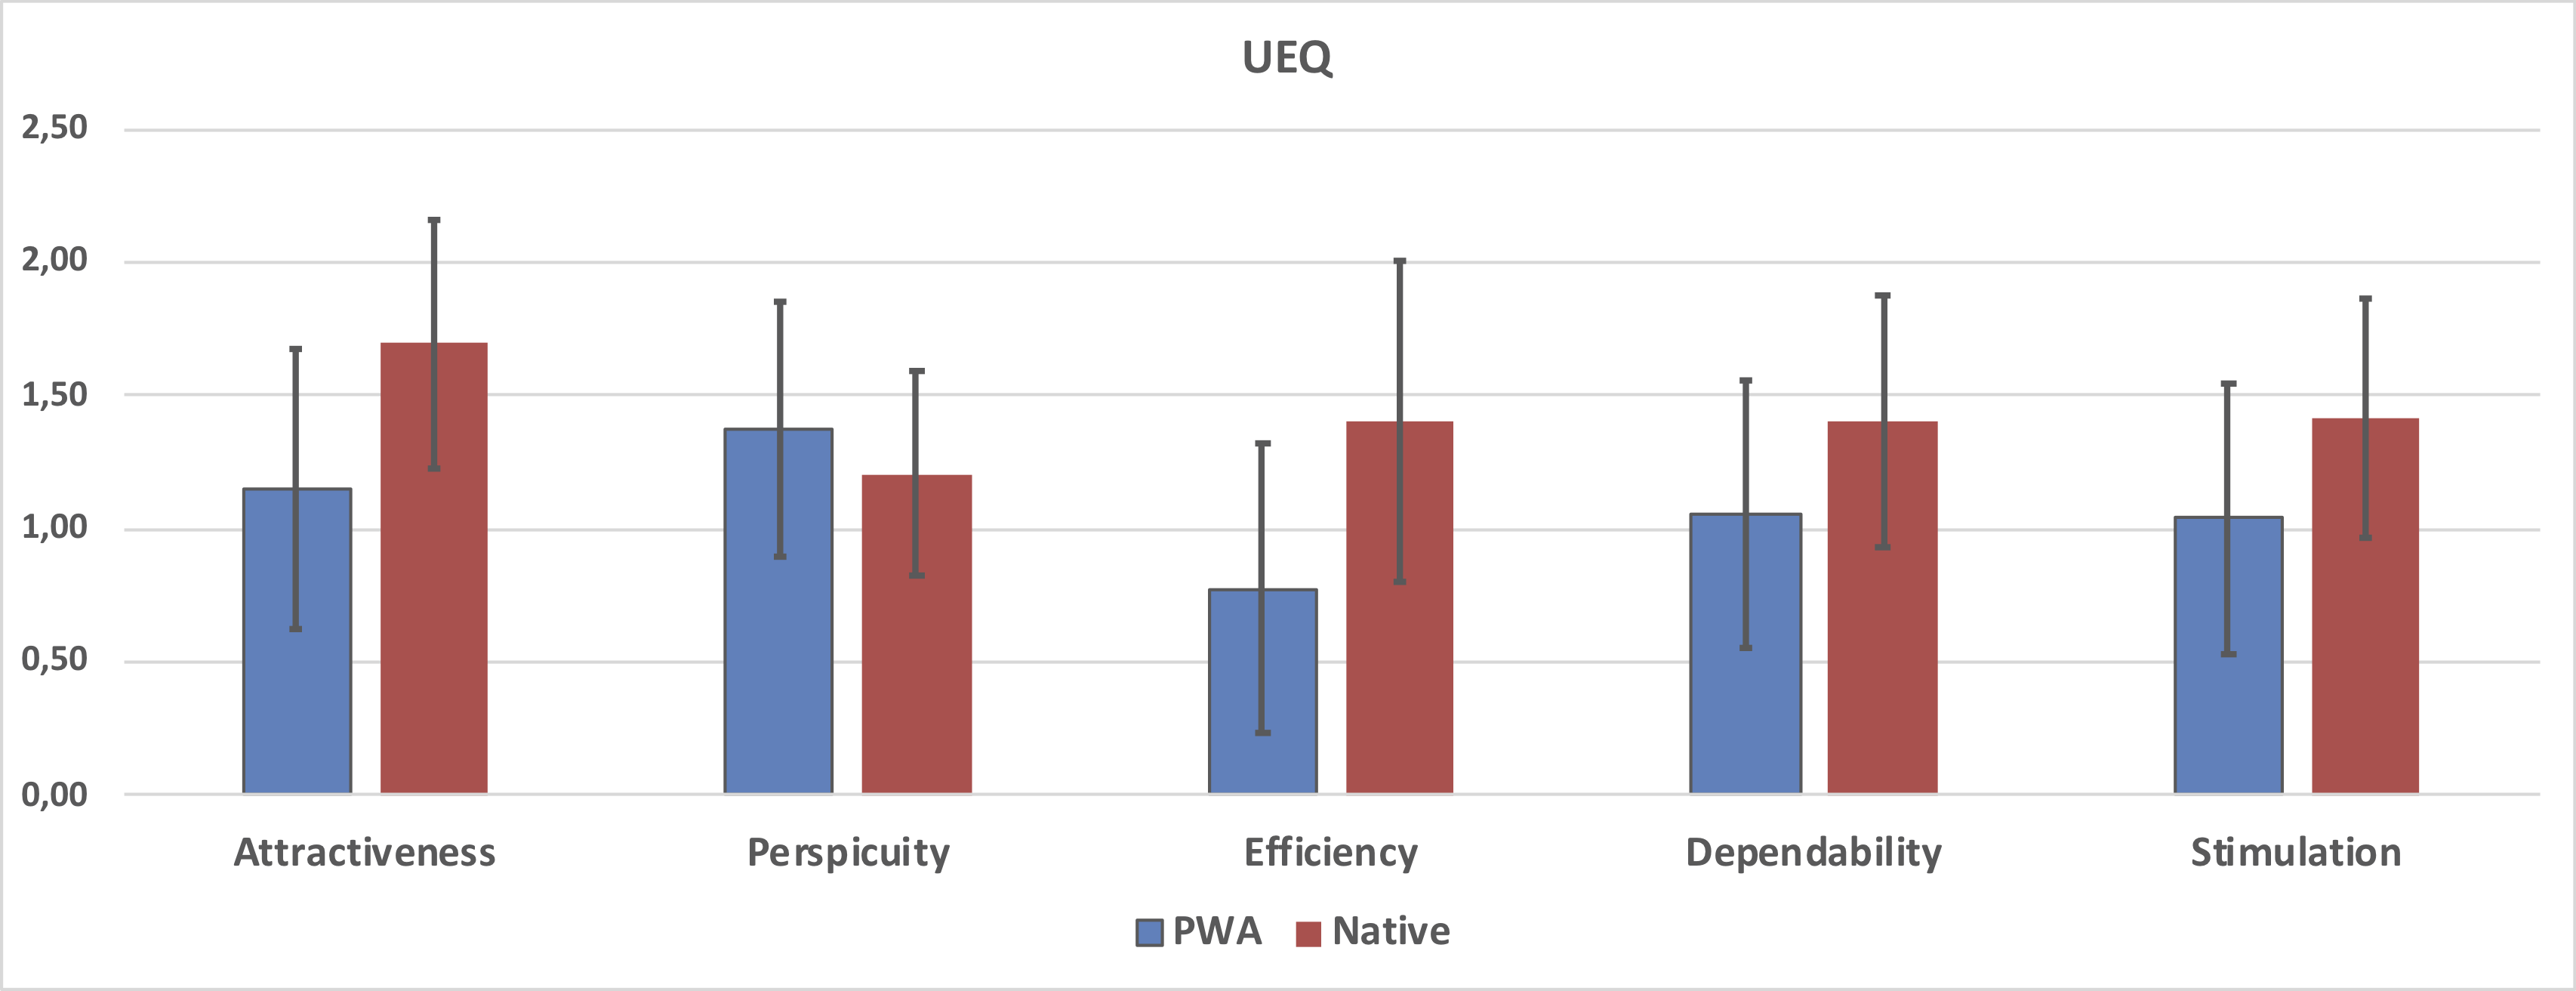
\includegraphics[width=0.99\textwidth]{img/UEQ_Result.png}
    \hfill
    \caption{\label{fig:ueq-result}{UEQ results from Usability Test}}
\end{figure}

\subsubsection{SUS}

The result from the SUS, seen in figure \ref{fig:sus-comparison} indicated that Android users preferred the Native application, whereas iPhone users preferred the PWA. However, these results were not statistically significant and were therefore not included in the calculations for the model.

\begin{figure}[ht]
    \centering 
    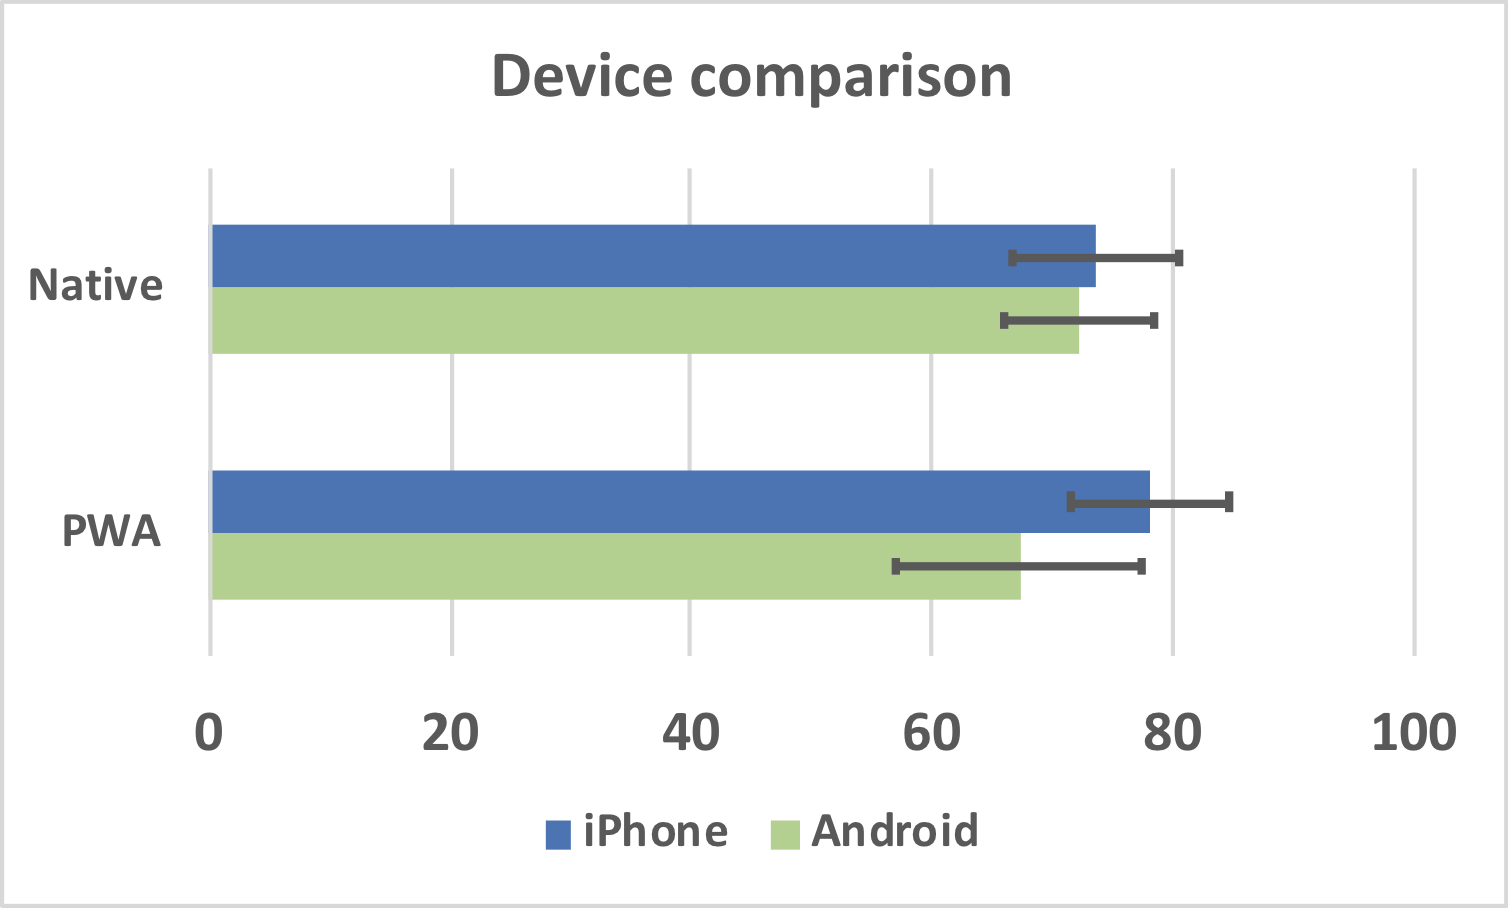
\includegraphics[width=0.8\textwidth]{img/SUS-Comparison.png}
    \hfill
    \caption{\label{fig:sus-comparison}{A SUS-Score comparison between iPhone and Android for PWA and Native.}}
\end{figure}

\subsubsection{Qualitative data}

The result from the qualitative questions after the Usability tests, and the responses and reactions recorded in written form at the test sessions, produced the first iteration of qualitative data.

10 subjects said that they experienced the PWA to be slow or slower in comparison with the native application. 2 subjects expressed that the native application was slow.

3 subjects said that they found the PWA to be easier to navigate. No such opinion was expressed about the native application.

3 subjects said the PWA felt like a web page or felt "web-like".

5 subjects had visible trouble with the search bar in the PWA due to poor responsiveness. 1 subject had similar problems with the native application. 2 subjects vocally expressed problems with the hitbox-size of the native applications buttons.

6 subjects noted the native applications was more attractive, 2 subjects preferred the aesthetic of the PWA.

The iPhone users more often preferred the layout of the PWA, 3 out of 5 subjects using iPhones preferred the PWA on the aspects of user interface.

3 subjects preferred native even though they liked the user interface of PWA more, due to the poor responsiveness of the PWA.


\subsection{Model}

The model was implemented with \textit{Vue.js}. The dependencies added for this implementation were \textit{Chart.js} for creating bar-charts, a slider component for the ranking, \textit{Vuetify} for the styling, \textit{Vue-router} and \textit{Vuex} for functionality like saving state and swapping between different views. The code for the implementation can be found on the following GitHub repository: 
\textit{\href{https://github.com/sebastian-porling/mobile\_application\_mcdm}{https://github.com/sebastian-porling/mobile\_application\_mcdm}}. 

The implementation consisted of three parts. The first view seen in figure \ref{fig:implementation_views:1} was a form, which gathered the functions that were needed for the application and some follow up questions. The second view seen in figure \ref{fig:implementation_views:2} was used for ranking the different criteria. The slider made the ranking more perspicuous. The ranking could have been implemented in many ways, like filling in a number for each criterion, but this version made it easier to see the relationship between the criteria. The final view seen in figure \ref{fig:implementation_views:3} was the result of the calculation. It gave the recommended alternative for the decision-maker, showed how much better the alternative is compared to the other alternatives and gave a bar chart that showed how much the score was affected by the different criteria. A list of functions which will not be available while using PWA was presented. 

\begin{figure}[ht]
	\centering 
	\subfloat[The form]{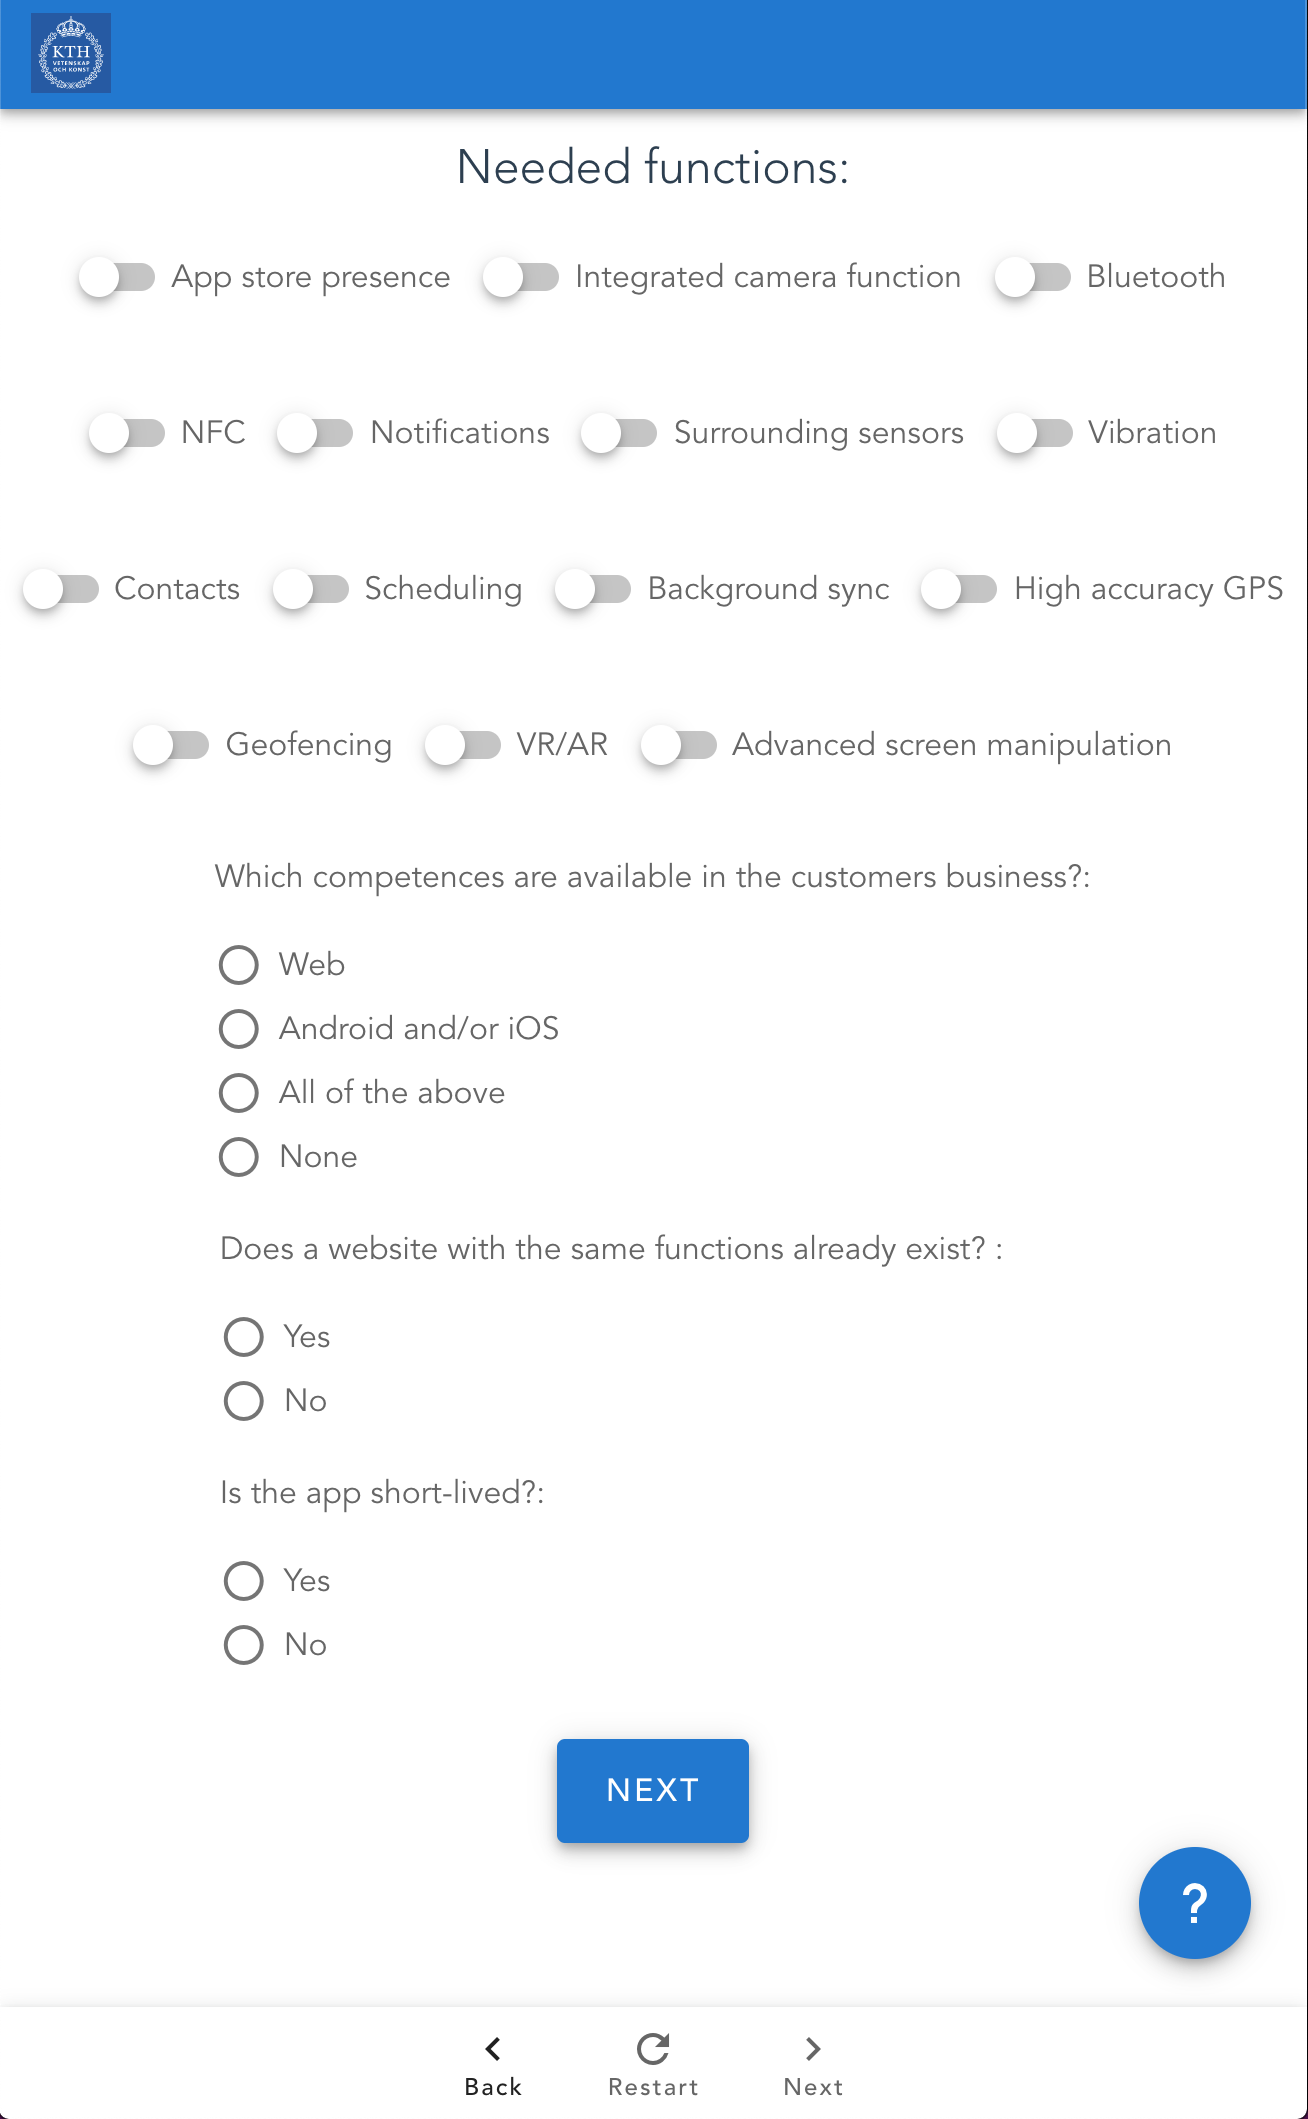
\includegraphics[width=0.45\textwidth]{img/implementation_form_view.png}
		\label{fig:implementation_views:1}}
	\hfill
	\subfloat[Ranking module]{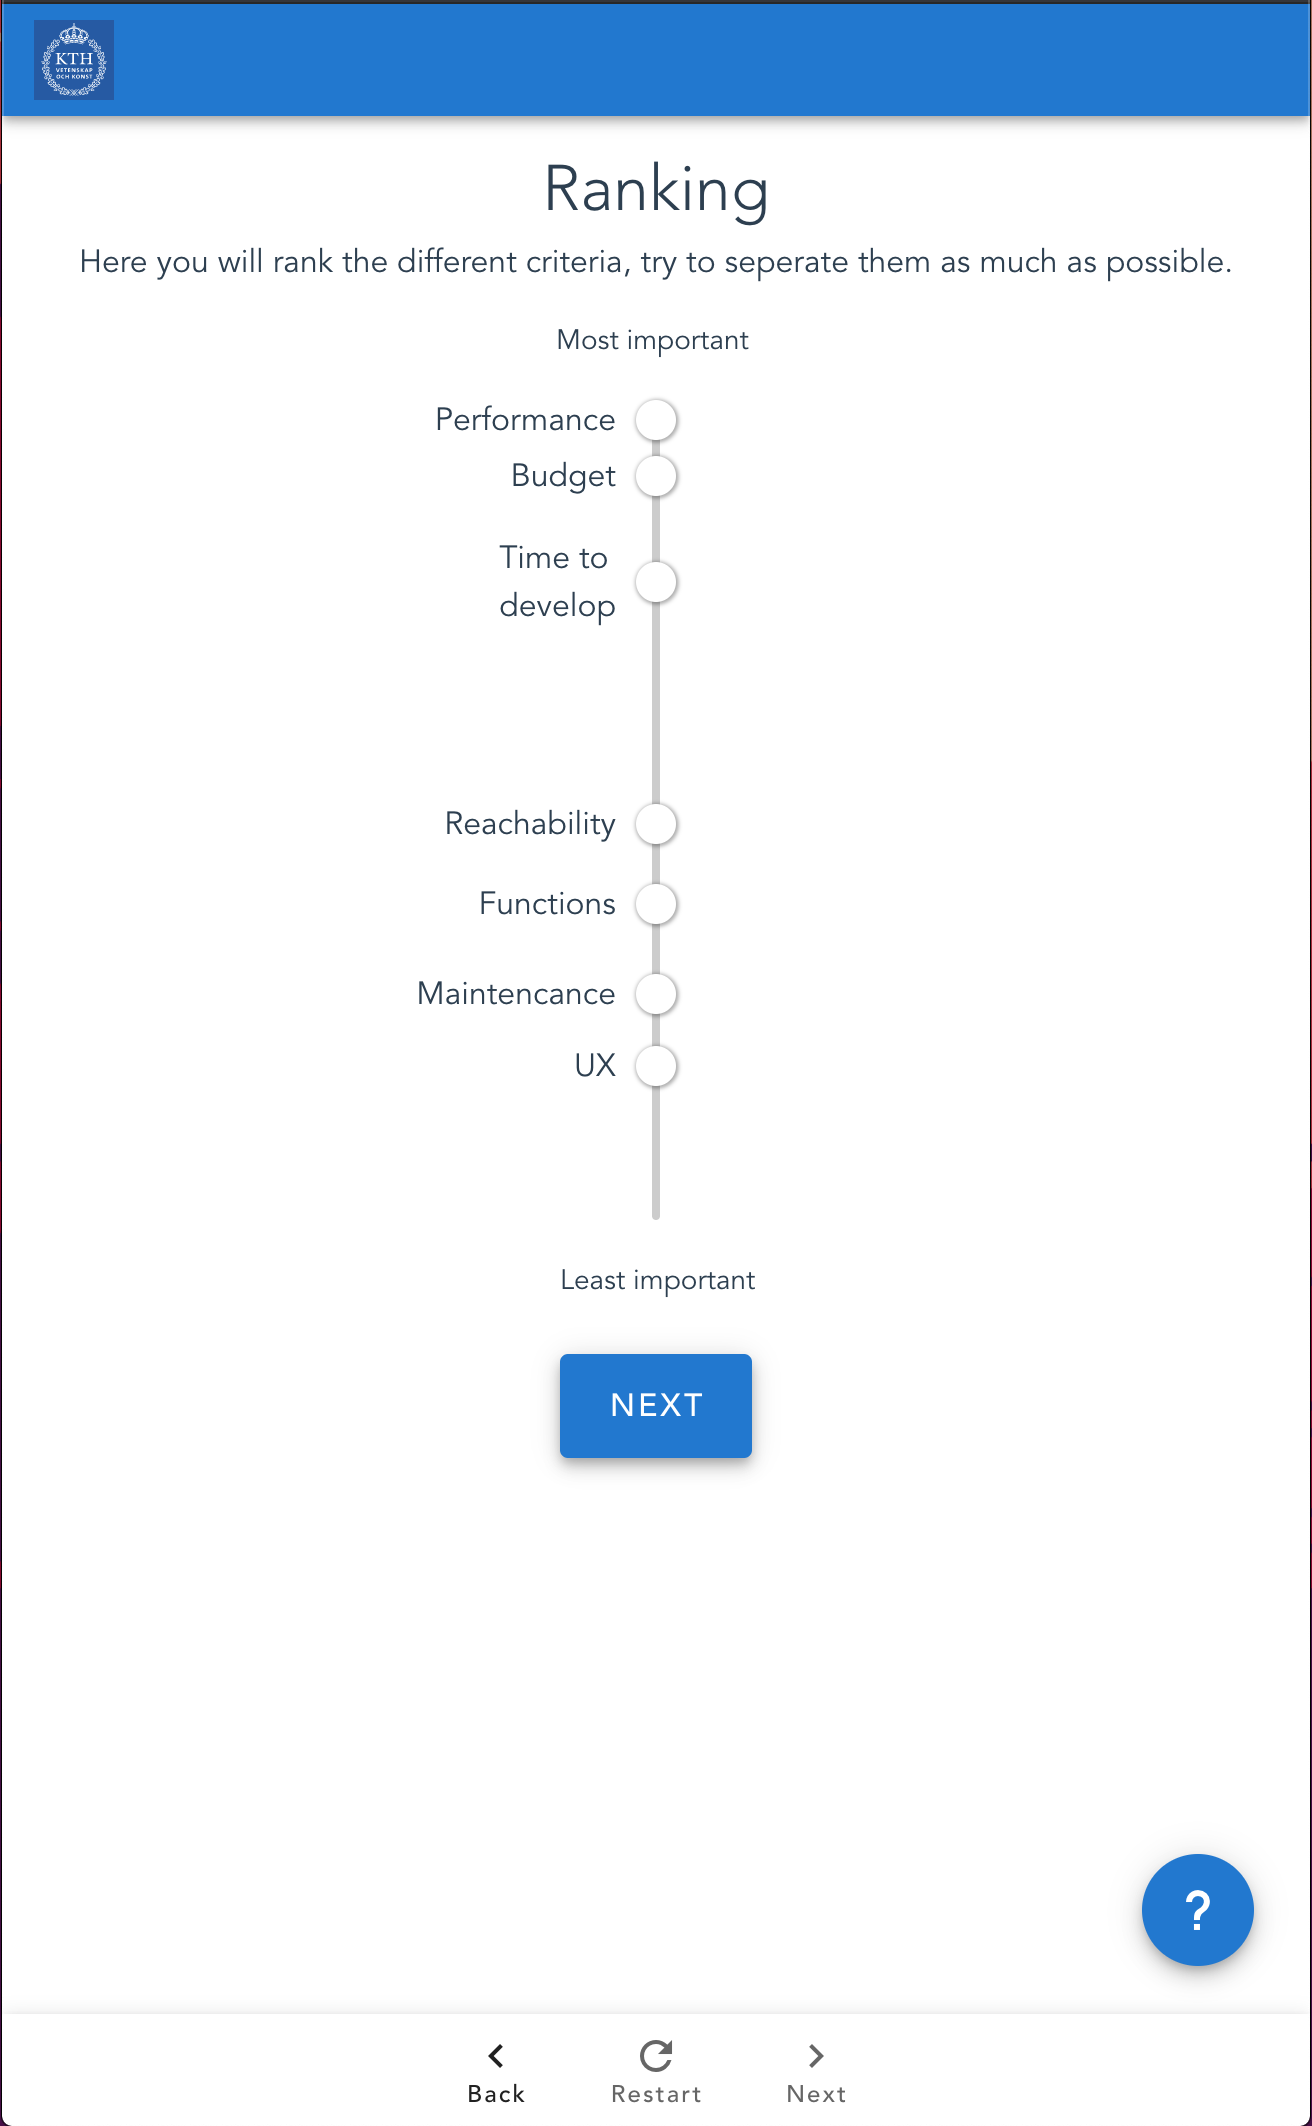
\includegraphics[width=0.45\textwidth]{img/implementation_ranking_view.png}
		\label{fig:implementation_views:2}}
	\hfill
	\subfloat[Result view with graph]{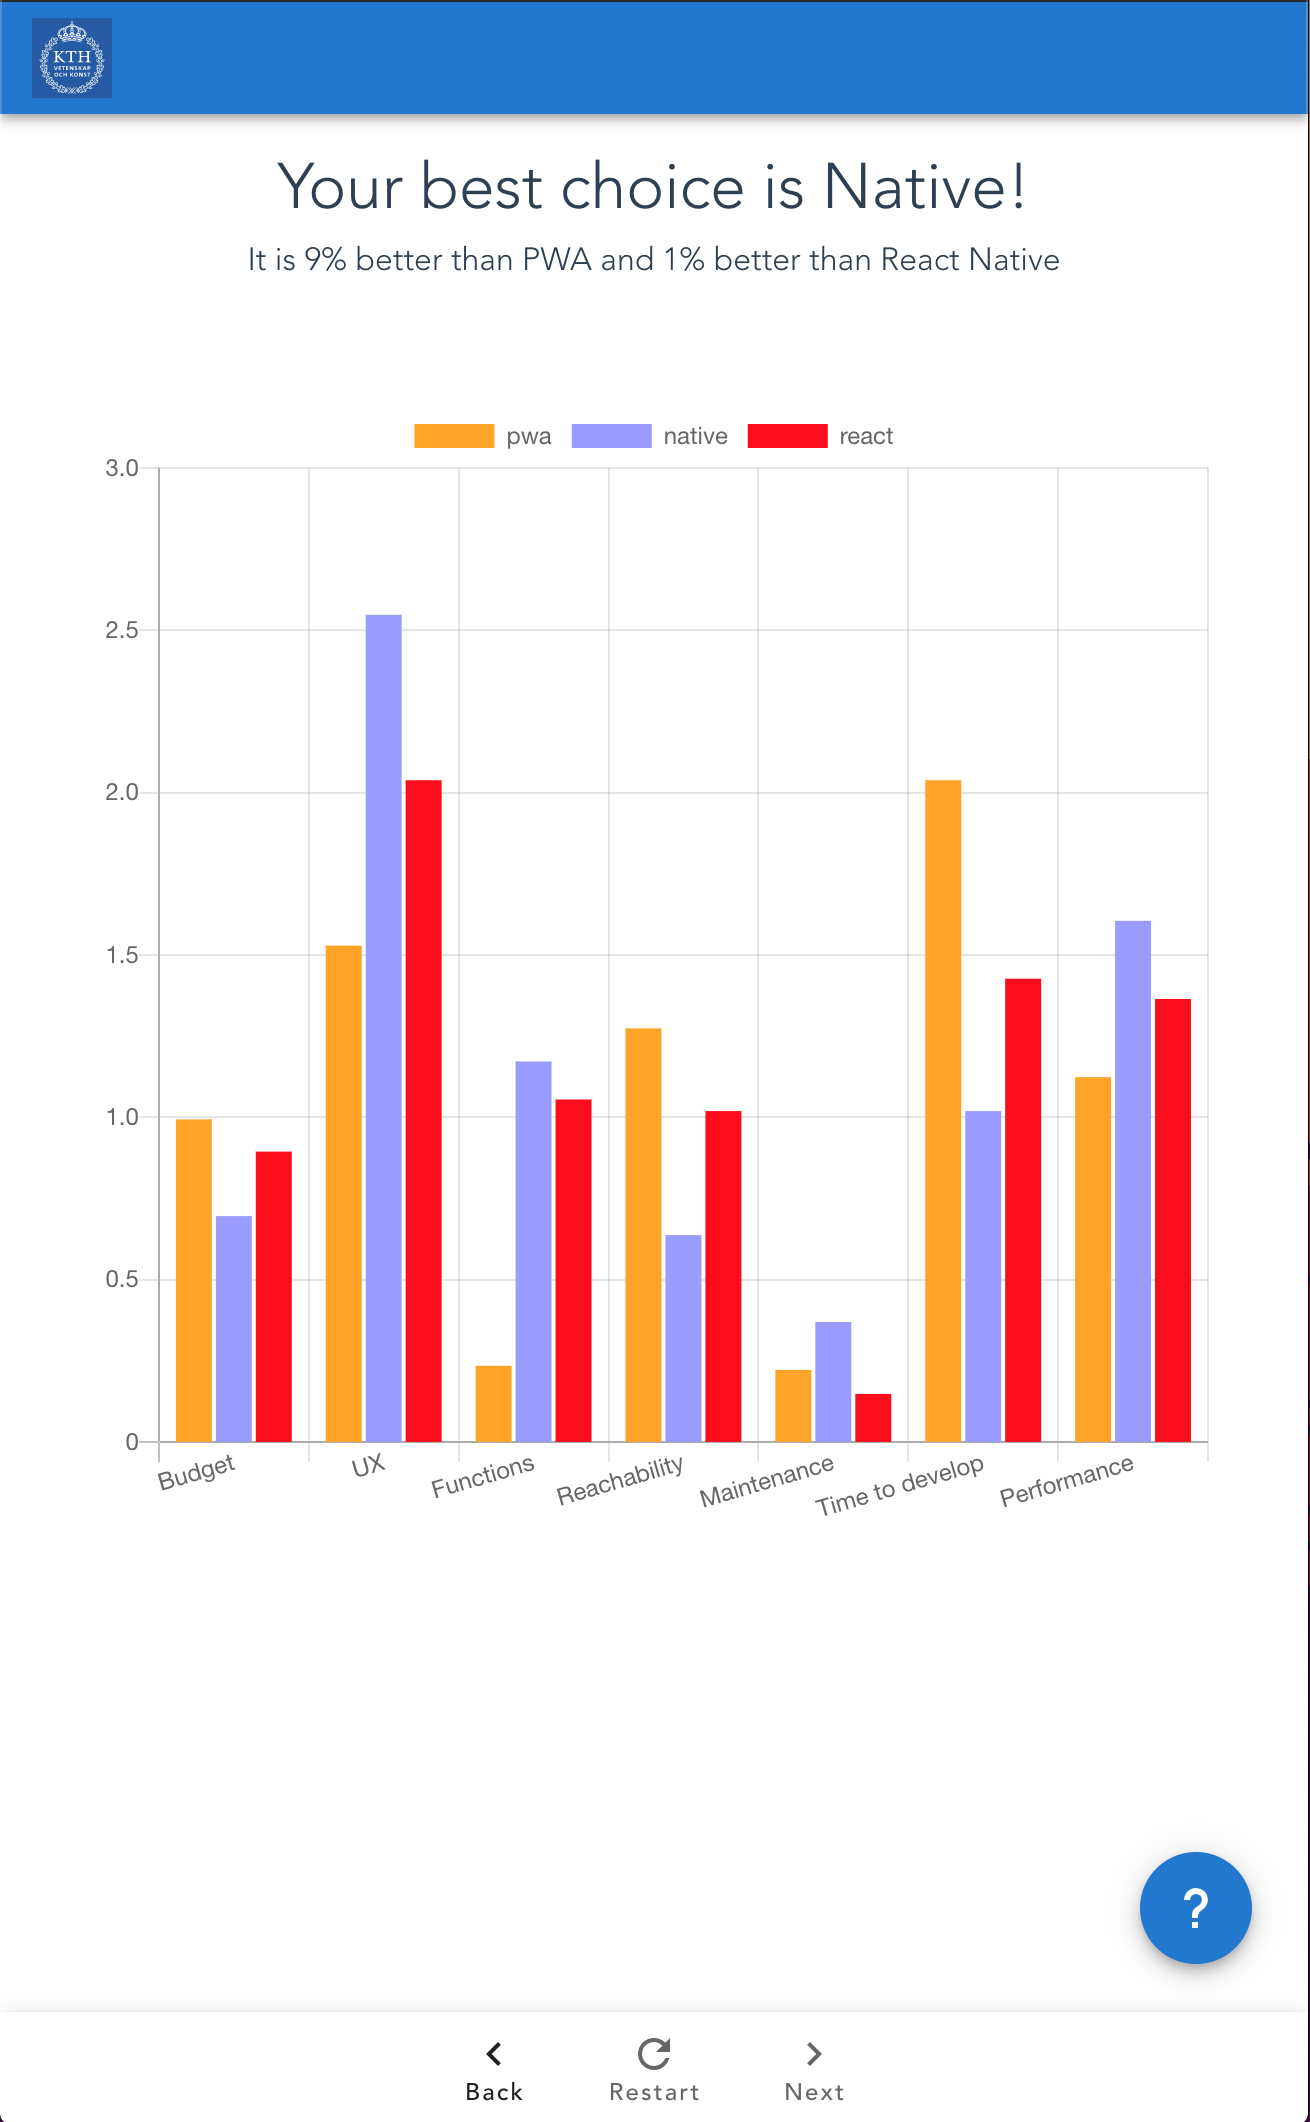
\includegraphics[width=0.45\textwidth]{img/implementation_result_view.png}
		\label{fig:implementation_views:3}}
	\caption{\textit{Screenshots of the different views for the implementation.}}
\end{figure}
